% Additional TikZ Diagrams for Part I
% Generated automatically

% ============================================
% Bloom Filter Detailed
% ============================================

% Bloom Filter Bit Array with Hash Functions
\begin{figure}[h]
\centering
\begin{tikzpicture}[scale=0.7]
    % Define bit array size
    \def\bits{32}
    
    % Draw bit array
    \foreach \i in {0,...,31} {
        \pgfmathtruncatemacro{\bitval}{mod(\i,3)==0 || mod(\i,7)==0 ? 1 : 0}
        \ifnum\bitval=1
            \node[rectangle, draw, fill=green!30, minimum size=0.5cm] at (\i*0.55,0) {\tiny 1};
        \else
            \node[rectangle, draw, fill=white, minimum size=0.5cm] at (\i*0.55,0) {\tiny 0};
        \fi
    }
    
    % Add labels
    \node[below] at (8.5,-0.5) {Bit Array (m = 32 bits)};
    
    % Show hash functions mapping
    \node[draw, rounded corners, fill=blue!20] (elem) at (4,2.5) {Element: "apple"};
    
    % Hash function arrows
    \draw[->, thick, red] (elem) -- (2.2,0.5) node[midway, left] {$h_1$};
    \draw[->, thick, blue] (elem) -- (6.6,0.5) node[midway] {$h_2$};
    \draw[->, thick, green!50!black] (elem) -- (10.45,0.5) node[midway, right] {$h_3$};
    
    % Statistics box
    \node[draw, align=left] at (14,2) {
        \textbf{Parameters:}\\
        m = 32 bits\\
        k = 3 hash functions\\
        n = 10 elements\\
        FP rate ≈ 0.054
    };
\end{tikzpicture}
\caption{Bloom filter: Multiple hash functions map elements to bit positions}
\label{fig:bloom-detail}
\end{figure}


% ============================================
% Query Pattern Heatmap
% ============================================

% Query Pattern Heatmap
\begin{figure}[h]
\centering
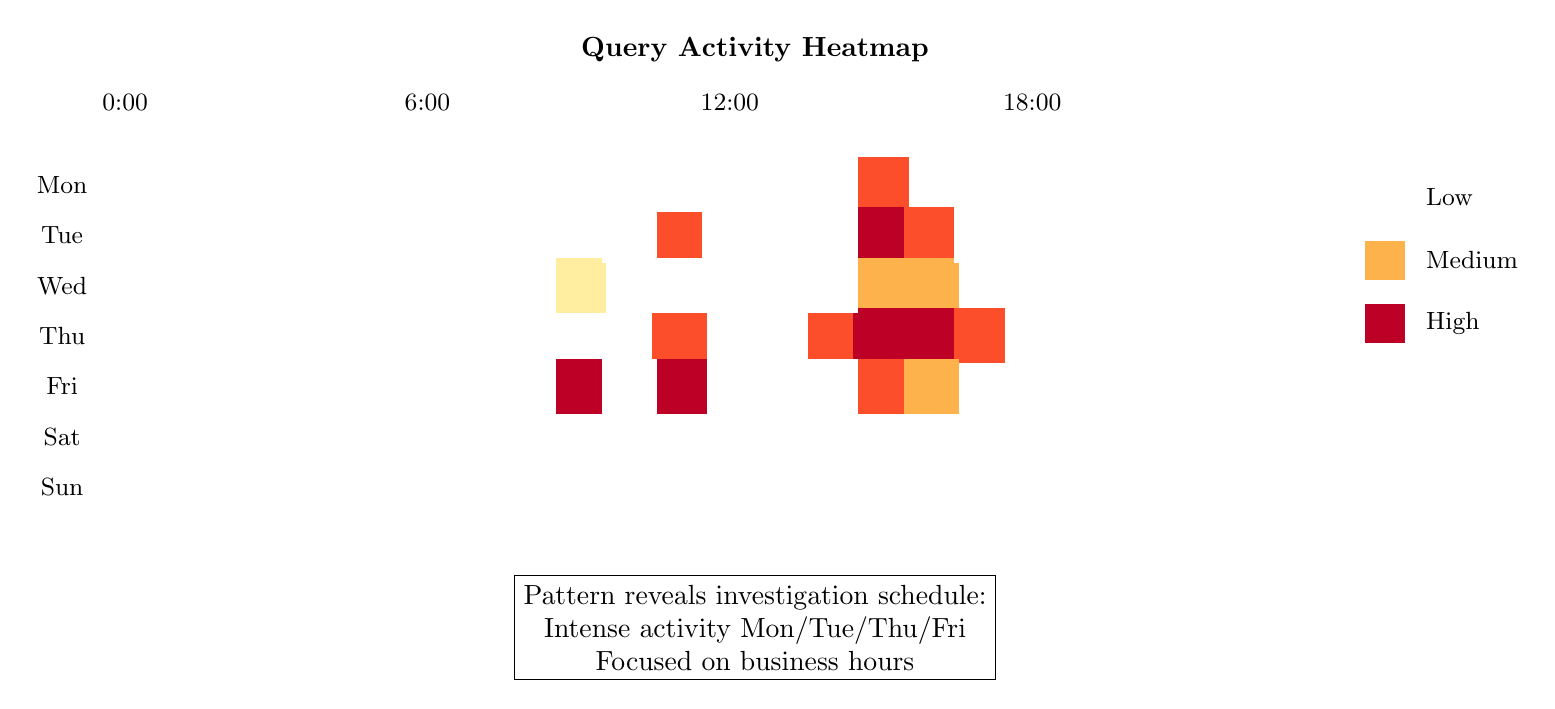
\begin{tikzpicture}[scale=0.8]
    % Define heatmap colors
    \definecolor{heat0}{RGB}{255,255,255}
    \definecolor{heat1}{RGB}{255,237,160}
    \definecolor{heat2}{RGB}{254,178,76}
    \definecolor{heat3}{RGB}{252,78,42}
    \definecolor{heat4}{RGB}{189,0,38}
    
    % Days of week
    \foreach \d [count=\di] in {Mon,Tue,Wed,Thu,Fri,Sat,Sun} {
        \node at (-1, -\di*0.8) {\small \d};
    }
    
    % Hours
    \foreach \h in {0,6,12,18} {
        \node at (\h*0.8, 0.5) {\small \h:00};
    }
    
    % Heatmap data (journalist pattern - focused bursts)
    % Monday
    \foreach \h/\intensity in {9/3,10/4,11/4,14/2,15/3} {
        \node[rectangle, fill=heat\intensity, minimum size=0.7cm] at (\h*0.8, -1*0.8) {};
    }
    
    % Tuesday
    \foreach \h/\intensity in {10/2,11/3,14/4,15/4,16/3} {
        \node[rectangle, fill=heat\intensity, minimum size=0.7cm] at (\h*0.8, -2*0.8) {};
    }
    
    % Wednesday
    \foreach \h/\intensity in {9/1,15/2,16/2} {
        \node[rectangle, fill=heat\intensity, minimum size=0.7cm] at (\h*0.8, -3*0.8) {};
    }
    
    % Thursday
    \foreach \h/\intensity in {11/3,14/3,15/4,16/4,17/3} {
        \node[rectangle, fill=heat\intensity, minimum size=0.7cm] at (\h*0.8, -4*0.8) {};
    }
    
    % Friday
    \foreach \h/\intensity in {9/4,10/4,11/4,14/3,15/3,16/2} {
        \node[rectangle, fill=heat\intensity, minimum size=0.7cm] at (\h*0.8, -5*0.8) {};
    }
    
    % Fill remaining with low intensity
    \foreach \di in {1,...,7} {
        \foreach \h in {0,...,23} {
            \pgfmathtruncatemacro{\show}{random(0,1)}
            \ifnum\show=1
                \node[rectangle, fill=heat0, minimum size=0.7cm] at (\h*0.8, -\di*0.8) {};
            \fi
        }
    }
    
    % Title and legend
    \node[above] at (10, 1) {\textbf{Query Activity Heatmap}};
    
    % Legend
    \node[rectangle, fill=heat0, minimum size=0.5cm] at (20, -1) {};
    \node[right] at (20.5, -1) {\small Low};
    \node[rectangle, fill=heat2, minimum size=0.5cm] at (20, -2) {};
    \node[right] at (20.5, -2) {\small Medium};
    \node[rectangle, fill=heat4, minimum size=0.5cm] at (20, -3) {};
    \node[right] at (20.5, -3) {\small High};
    
    % Annotation
    \node[draw, align=center, below] at (10, -7) {
        Pattern reveals investigation schedule:\\
        Intense activity Mon/Tue/Thu/Fri\\
        Focused on business hours
    };
\end{tikzpicture}
\caption{Query patterns reveal user behavior and intent}
\label{fig:query-heatmap}
\end{figure}


% ============================================
% Encoding Comparison
% ============================================

% Oblivious Encoding Comparison
\begin{figure}[h]
\centering
\begin{tikzpicture}[scale=1.1]
    % Traditional path
    \node[draw, rectangle] (trad_input) at (0,3) {Query: "covid"};
    \node[draw, rectangle, fill=blue!20] (trad_hash) at (3,3) {SHA256};
    \node[draw, rectangle] (trad_output) at (6,3) {0x3f2a8b...};
    \node[draw, ellipse, fill=red!20] (trad_pattern) at (9,3) {Pattern\\Visible};
    
    \draw[->] (trad_input) -- (trad_hash);
    \draw[->] (trad_hash) -- (trad_output);
    \draw[->, dashed, red] (trad_output) -- (trad_pattern);
    
    \node[above] at (3,3.5) {\textbf{Traditional}};
    
    % Oblivious path
    \node[draw, rectangle] (obl_input) at (0,0) {Query: "covid"};
    \node[draw, rectangle, fill=green!20] (obl_encode) at (2.5,0) {Bernoulli\\Encode};
    \node[draw, cloud, cloud puffs=10, fill=gray!20] (obl_noise) at (5.5,0) {Uniform\\Noise};
    \node[draw, ellipse, fill=green!20] (obl_private) at (9,0) {No\\Pattern};
    
    \draw[->] (obl_input) -- (obl_encode);
    \draw[->] (obl_encode) -- (obl_noise);
    \draw[->, dashed, green!50!black] (obl_noise) -- (obl_private);
    
    \node[below] at (3,-0.5) {\textbf{Oblivious}};
    
    % Comparison arrows
    \draw[<->, thick, red] (9,2.3) -- (9,0.7) node[midway, right] {Privacy\\Gap};
    
    % Adversary
    \node[draw, ellipse, fill=gray!30] (adversary) at (11,1.5) {Adversary};
    \draw[->, red] (trad_pattern) -- (adversary);
    \draw[->, dashed, gray] (obl_private) -- (adversary);
    
    % Annotations
    \node[align=left] at (11,-1) {
        \textcolor{red}{✗ Frequency analysis}\\
        \textcolor{red}{✗ Correlation attacks}\\
        \textcolor{green!50!black}{✓ Indistinguishable}
    };
\end{tikzpicture}
\caption{Traditional vs. Oblivious encoding: Achieving privacy through uniformity}
\label{fig:encoding-comparison}
\end{figure}


% ============================================
% Error Composition Tree
% ============================================

% Error Composition Tree
\begin{figure}[h]
\centering
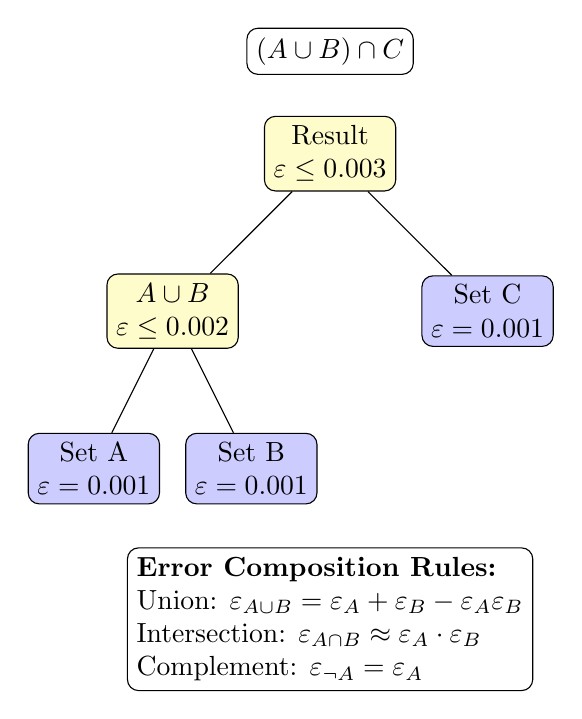
\begin{tikzpicture}[
    level distance=2cm,
    level 1/.style={sibling distance=4cm},
    level 2/.style={sibling distance=2cm},
    every node/.style={draw, rectangle, rounded corners, align=center},
    leaf/.style={fill=blue!20},
    op/.style={fill=yellow!20}
]
    \node[op] {Result\\$\varepsilon \leq 0.003$}
        child {
            node[op] {$A \cup B$\\$\varepsilon \leq 0.002$}
            child {
                node[leaf] {Set A\\$\varepsilon = 0.001$}
            }
            child {
                node[leaf] {Set B\\$\varepsilon = 0.001$}
            }
        }
        child {
            node[leaf] {Set C\\$\varepsilon = 0.001$}
        };
    
    % Operation label
    \node[above] at (0,1) {$(A \cup B) \cap C$};
    
    % Formula box
    \node[draw, align=left, below] at (0,-5) {
        \textbf{Error Composition Rules:}\\
        Union: $\varepsilon_{A \cup B} = \varepsilon_A + \varepsilon_B - \varepsilon_A \varepsilon_B$\\
        Intersection: $\varepsilon_{A \cap B} \approx \varepsilon_A \cdot \varepsilon_B$\\
        Complement: $\varepsilon_{\neg A} = \varepsilon_A$
    };
\end{tikzpicture}
\caption{Error propagation through Boolean operations}
\label{fig:error-tree}
\end{figure}


% ============================================
% System Architecture Detailed
% ============================================

% Detailed System Architecture
\begin{figure}[h]
\centering
\begin{tikzpicture}[scale=0.9,
    comp/.style={draw, rectangle, rounded corners, minimum width=2.5cm, minimum height=0.8cm},
    data/.style={draw, cylinder, shape border rotate=90, minimum width=2cm, minimum height=1cm},
    sec/.style={fill=red!20},
    proc/.style={fill=blue!20},
    stor/.style={fill=green!20}
]
    % Client Layer
    \node[comp] (app) at (0,5) {Application};
    \node[comp, proc] (parser) at (0,4) {Query Parser};
    \node[comp, proc] (encoder) at (0,3) {Bernoulli Encoder};
    \node[comp, sec] (crypto) at (0,2) {Crypto Layer};
    
    % Network
    \node[cloud, draw, cloud puffs=12, minimum width=3cm] (net) at (4,2.5) {TLS/Network};
    
    % Server Layer
    \node[comp, sec] (auth) at (8,5) {Authentication};
    \node[comp, proc] (handler) at (8,4) {Request Handler};
    \node[comp, proc] (engine) at (8,3) {Oblivious Engine};
    \node[data, stor] (bloom) at (8,1.5) {Bloom Storage};
    \node[data, stor] (index) at (10.5,1.5) {Index};
    
    % Connections
    \draw[->] (app) -- (parser);
    \draw[->] (parser) -- (encoder);
    \draw[->] (encoder) -- (crypto);
    \draw[<->] (crypto) -- (net);
    \draw[<->] (net) -- (auth);
    \draw[->] (auth) -- (handler);
    \draw[->] (handler) -- (engine);
    \draw[<->] (engine) -- (bloom);
    \draw[<->] (engine) -- (index);
    
    % Security boundaries
    \draw[dashed, red, thick] (-1.5,1) rectangle (1.5,5.5);
    \node[red] at (0,0.5) {Trusted Client};
    
    \draw[dashed, red, thick] (6.5,0.5) rectangle (11.5,5.5);
    \node[red] at (9,0) {Untrusted Server};
    
    % Privacy guarantee
    \node[draw, align=center, fill=yellow!20] at (4,5) {
        \textbf{Privacy Guarantee:}\\
        Server learns nothing\\
        about query content
    };
\end{tikzpicture}
\caption{Complete system architecture with security boundaries}
\label{fig:system-detailed}
\end{figure}


